\documentclass[dvipdfmx]{jsarticle}
\usepackage[T1]{fontenc}
\usepackage[dvipdfmx]{hyperref}
\usepackage{lmodern}
\usepackage{latexsym}
\usepackage{amsfonts}
\usepackage{amssymb}
\usepackage{mathtools}
\usepackage{amsthm}
\usepackage{multirow}
\usepackage{graphicx}
\usepackage{wrapfig}
\usepackage{here}
\usepackage{float}
\usepackage{ascmac}
\usepackage{url}

\title{ネットワークプログラミングを利用したアプリケーション開発}
\date{\today}
\author{日本大学 文理学部情報科学科\\5419045 高林 秀}

\begin{document}

\maketitle

\begin{abstract}
本稿は、今年度発展プログラミングの課題研究としてProcessingを用いたネットワークプログラミングを使用したアプリケーション開発を行うものである。本稿前半部では、開発の際に利用した技術やコードに関して説明を行う。本稿後半部では、実際に説明した技術を用いて、Processing上で実行可能なアプリケーションを作成する。
\end{abstract}

\tableofcontents

\section{目的}
本稿の目的は、今年度発展プログラミングの課題研究としてProcessingを用いたネットワークプログラミングを使用したアプリケーション開発を行うものである。前半部にて基本的な技術用語の説明を通して、プログラミングの際に必要な知識の復習を行う。後半部では、実際にProcessing上で実行可能なアプリケーション開発を通してネットワークプログラミングを自身のプログラムに実装する。
\section{Processingの概要}
まず、本稿の開発言語であるProcessingに関して軽く触れる。\par
Processingは、オープンソースで開発されているプログラミング言語である。主に電子アートと、グラフィック・ビジュアルデザインに特化した機能を持ち合わせており、他のプログラミング言語よりも視覚的な表現とフィードバックを簡単に得れるという特徴を持つ。\par
この言語は、米国出身のCasey Reas氏とBenjamin Fry氏によって開発・設計された。Reas氏は、マサチューセッツ工科大学のMITメディアラボの美学および計算グループの一部として、メディアアートと科学の理学修士号を取得している人物であり、Fry氏は、データの視覚化に関する専門知識を持つアメリカ人デザイナーで、カーネギーメロン大学でコンピューターサイエンスの副専攻であるコミュニケーションデザインのBFAを取得し、修士号と博士号を取得している人物である。\par
Processingの構文は、Javaに似ており、Javaをより単純化した様な構文で構成される。開発の際には、skechbookと呼ばれる統合開発環境(IDE)を利用して行う。\par
\begin{figure}[H]
  \centering
  
\includegraphics[scale=0.4]{images/180px-Processing_Logo_Clipped.svg.png}
  \caption{Processingロゴ}
  出典:\url{https://ja.wikipedia.org/wiki/Processing}
\end{figure}
\section{ネットワークプログラミング概要}
この章では、開発に関連する基本的な技術用語の説明を簡単に行う。
\subsection{プロトコル}
コンピュータ同士がネットワークを介して通信を行うには、データの形式や送受信の手順を定めた「プロトコル」と呼ばれるルールのようなものが必要である。プロトコルにはいくつか種類があり同一のプロトコルに従っているコンピュータ同士のみネットワーク通信を行うことが可能だ。\par
単純なアプリケーション開発でも、ネットワーク通信を行うには様々な決め事(通信先の機器の指定、データ型の指定等)を定める必要があり、異常な手間がかかる。したがって実際にネットワークプログラミングを行う際には「プロトコルスタック」と呼ばれる、プロトコルを階層化した概念が取り入れられる。この理論的モデルが「OSI参照モデル」と呼ばれるもので、それを簡略化したモデルが「TCP/IP」と呼ばれるプロトコルスタックである。
\begin{figure}[H]
  \centering
  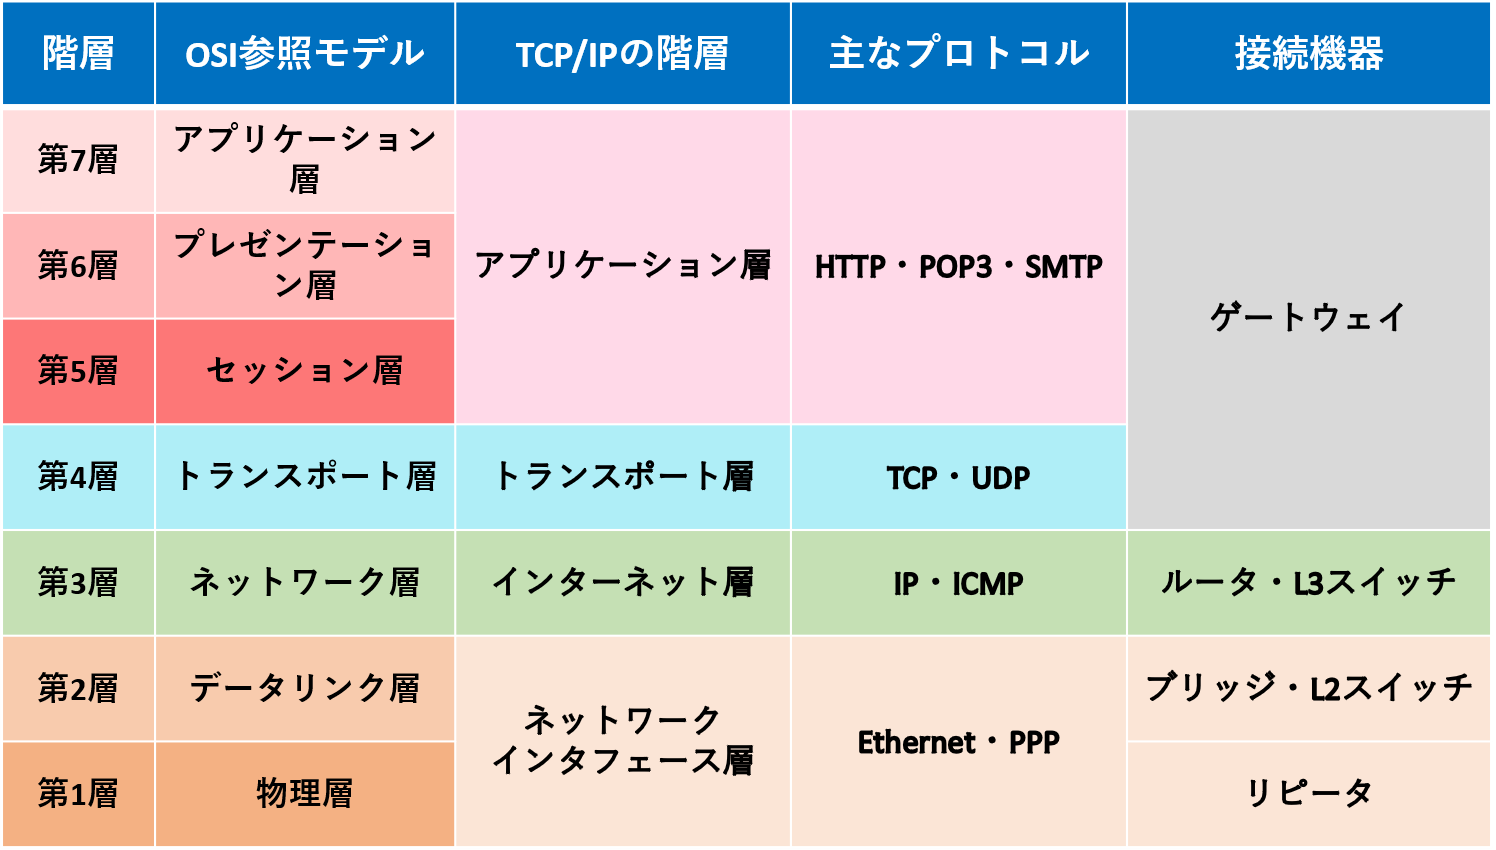
\includegraphics[scale=0.4]{images/ositcpip.png}
  \caption{OSI参照モデルとTCP/IP、その他プロトコルの関係図}
  出典:\url{https://ansl-blog.hatenablog.com/entry/2019/05/22/OSI%E5%8F%82%E7%85%A7%E3%83%A2%E3%83%87%E3%83%AB%E3%81%A8TCP%EF%BC%8FIP%E3%81%AB%E3%81%A4%E3%81%84%E3%81%A6}
\end{figure}
\subsection{TCP/IP}
TCP/IPは一般的にネットワークプロトコル群の総称を指し、接続先のコンピュータと通信を行うアプリケーションを指定するため、IPアドレスとポート番号を利用する。IPアドレスは、コンピュータの住所のようなもので、個別にコンピュータごとに割り当てられた文字列である。ポート番号は、通信を行うアプリケーションを指定する際に使用する。\par
前項の図の通り、OSI参照モデルでは細かく7層に通信機能が分類されているが、プログラミングを行う際には細かすぎるため実用的ではなかった。したがって、よりシンプルかつ実用的な階層構造にしたものがTCP/IPである。現代ののネットワーク通信ではこのTCP/IPが用いられている。
\subsection{Processingにおけるネットワークプログラミング}
Processingには、ネットワーク上のコンピュータ間でデータを読み書きするための機能が標準ライブラリとして準備されている。そのため、Processingの実行環境以外新たに外部からインストールするライブラリやモジュールは必要ない。\par
ネットワーク通信を行うためには当然だが、クライアントサイド(接続する側)とサーバーサイド(接続される側)双方にプログラムを用意する必要がある。そのための関連機能として、Processingには「processing.net」と呼ばれるライブラリが用意されている。\par
それぞれのサイドのプログラムを作成する際はこのライブラリをインポートする必要がある。\par
\begin{verbatim}
  import processing.net.*;
\end{verbatim}
各サイドで利用するメソッドやクラスの使用法は後述する章を参照いただきたい。
\section{クライアントサイド}
\subsection{ProcessingのClientクラス}
Processingにてクライアントサイドプログラムを実装するには、Clientクラスを使用する。このClientクラスを用いることで、後述するServerクラスを持つプログラムとTCP通信ができる。\par
Clientクラスは、3引数のコンストラクタを持っている。以下引数の概要を示す。
\begin{verbatim}
  Client(PApplet インスタンス, サーバーのIPアドレスorホスト名, サーバーのポート番号)
\end{verbatim}
\begin{enumerate}
  \item PApplet インスタンス:自身のインスタンスを示す「this」。
  \item サーバーのIPアドレスorホスト名:文字列(String)型。例:192.168.xx.x。
  \item サーバーのポート番号:サーバー側のアプリケーションを識別するためのポート番号。整数(int)型。
\end{enumerate}


\section{サーバーサイド}
\subsection{ProcessingのServerクラス}
前章のClientクラスと同様に、Processingでサーバーサイドプログラムを実装するには、Serverクラスを利用する。\par
このクラスは、2引数のコンストラクタを持っている。
\begin{verbatim}
  Client(PApplet インスタンス, 待機するポート番号)
\end{verbatim}
\begin{enumerate}
  \item PApplet インスタンス:自身のインスタンスを示す「this」。
  \item 待機するポート番号:クライアント側の通信を待機するポート番号。整数(int)型。
\end{enumerate}
\section{Processingのイベントハンドラ}
TCP通信を用いるプログラミングでは、サーバー接続時や、切断時など様々な場面のときに行う処理である「イベントハンドラ」を定義することができる。特にProcessingでは、次のイベントを利用することができる。\par
\begin{itemize}
  \item serverEvent:serverEvent()内のコードは、プログラム内に作成されたサーバーに新しいクライアントが接続されたときに実行される。
  \item clientEvent:サーバーが既存のクライアントオブジェクトに値を送信する際に呼び出される。
  \item disconnectEvent:クライアントとの接続が切れた際に呼び出される。
\end{itemize}
各イベントハンドラは、上記名前の関数を定義しその中に処理を記述する。
\begin{verbatim}
  void serverEvent(Server s, Clinet c) {
    //Do something....
  }
\end{verbatim}

\section{アプリケーション実装}
\subsection{開発環境}
今回の開発は仮想マシン上で行った。下記に当時の環境を示す。
\begin{itemize}
  \item ホストOS:Window10 Home 20H2
  \item 仮想OS:Ubuntu 20.04.2 LTS
  \item CPU:Intel(R)Core(TM)i7-9700K @ 3.6GHz
  \item GPU:Nvidia Geforce RTX2070 OC @ 8GB
  \item ホストRAM:16GB
  \item 仮想RAM:4GB
  \item Processing version : 3.5.3
\end{itemize}
\subsection{制作内容}
下記に制作物の概要を示す。
\begin{itemize}
  \item 制作物名称:プロひげ危機一髪!!
  \item 名称の由来:本アプリ開発言語であるProcessingの「プロ(Pro)」と大人気ゲーム「黒ひげ危機一髪\footnote{黒ひげ危機一発(英名:Pop-up Pirate):1975年にタカラトミー(旧名:トミー)から発売されたゲーム玩具。海賊が頭だけを出している樽に対して短剣を刺し、樽から飛び出す海賊の反応を楽しむゲーム。}」を模したアプリケーションであることに由来する。
  \begin{figure}[H]
    \centering
    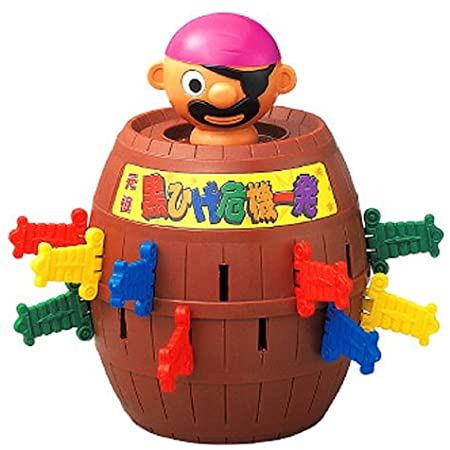
\includegraphics[scale=0.2]{images/51FOE881fOL._AC_SS450_.jpg}
    \caption{黒ひげ危機一髪}
    出典:\url{https://www.amazon.co.jp/%E3%82%BF%E3%82%AB%E3%83%A9%E3%83%88%E3%83%9F%E3%83%BC-TAKARA-TOMY-%E9%BB%92%E3%81%B2%E3%81%92%E5%8D%B1%E6%A9%9F%E4%B8%80%E7%99%BA/dp/B0002U3IRU}
  \end{figure}
  \item ルール
  \begin{enumerate}
    \item プレイヤーは、1~9の数値間でキー入力を行う。
    \item ランダムで決定されたある特定の数字をプレイヤーが入力した場合、そのプレイヤーの負けとなる。
    \item 上記以外の場合はセーフ。
  \end{enumerate}
\end{itemize}
\subsection{ソースコード}
本アプリケーションのソースコードを下記に記載するが、巻末資料にあるリンクからも閲覧、ダウンロードできる。
\begin{itemize}
  \item client.pde
  \begin{verbatim}
    import processing.net.*;

    Client client;
    Bom bom;


    void setup(){
      size(600, 600);
      client = new Client(this, "127.0.1.1", 5500);
      bom = new Bom(width/2, height/2, 100, 100);
    }

    void draw() {
      background(255);
      bom.drawBom();

      if(bom.isFire) {
        bom.fireBom();
      }
    }


    void keyPressed() {
      client.write(key);
    }

    /*サーバーから値を受け取るイベントリスナー*/
    void clientEvent(Client client) {
       while(client.available() > 0) {
         String v = client.readString().trim();
         print(v);
         if(v == "BOM!!!") {//isFireがTrueにならないため。。。。

             bom.fireBom();
         }
       }
    }

    public class Bom {

      private float x, y, bom_width, bom_height;
      public boolean isFire;
      private Particle[] particleArray;

      Bom(float x, float y, float w, float h) {
        this.x = x;
        this.y = y;
        this.bom_width = w;
        this.bom_height = h;
        this.isFire = false;
        this.particleArray = new Particle[100];
      }

      void drawBom() {
        fill(0);
        noStroke();
        ellipse(this.x, this.y, this.bom_width, this.bom_height);
      }

      void fireBom(){
        for(int i = 0; i < particleArray.length; i++) {
          float px = random(width);
          float py = random(height);
          float pl = random(50);
          this.particleArray[i] = new Particle(px,py,pl,pl);
          this.particleArray[i].drawPrticle();
        }
      }
    }

    public class Particle {
      float x, y, w, h, mx, my;
      int bwColor;
      Particle(float x, float y, float w, float h) {
        this.x = x;
        this.y = y;
        this.w = w;
        this.h = h;
        this.mx = 2.0;
        this.my = 2.0;
        this.bwColor = int(random(255));
      }

      void drawPrticle() {
        if(this.x < 0 || this.x > width) {
          this.mx *= -1.0;
        }
        if(this.y < 0 || this.y > height) {
          this.my *= -1.0;
        }
        fill(this.bwColor);
        noStroke();
        ellipse(this.x, this.y, this.w, this.h);
        this.x += this.mx;
        this.y += this.my;
      }
    }
  \end{verbatim}
  \item server.pde
  \begin{verbatim}
      import processing.net.*;

      Server server;
      DetLoseNum loseNum;


      void setup() {
        server = new Server(this, 5500);
        loseNum = new DetLoseNum(1,10);
      }

      void draw() {
        background(255);
      }


      /*サーバー接続時*/
      void serverEvent(Server server, Client client) {
        println("HELLO WORLD");
        print(loseNum.loseNumber);
      }

      /*クライアントから値を受け取る時*/
      void clientEvent(Client client) {
         while(client.available() > 0) {
           int v = 0;
           v = int(client.readString().trim());
           println("clientInput:" + v);
           if(v == loseNum.loseNumber) {
             server.write("BOM!!!");
           }
         }
      }



      public class DetLoseNum {
        private int upper;
        private int lower;
        public int loseNumber;

        DetLoseNum(int upper, int lower) {
          this.upper = upper;
          this.lower = lower;
          this.assignment();
        }

        void assignment() {
          this.loseNumber = int(random(this.upper, this.lower));
        }
      }
  \end{verbatim}
\end{itemize}
\subsection{プログラム挙動説明}
\paragraph{client.pde}
作成したクラスの概要は以下の通り。
\begin{itemize}
  \item Bomクラス\par
  起動時に表示する爆弾役の黒円のオブジェクト。このクラスはコンストラクタで、描画位置のx,y座標、描画の縦横幅の値を決める。そしてメソッドとして、インスタンスから実際にオブジェクトを描画するdrawBom()メソッド、爆発演出を行うfireBom()メソッドを持っている。fireBom()メソッド内部には、小さな円を指定数描画し、ランダムに動かすParticleクラスのインスタンスを複数個生成し、関連するメソッドを呼び出すことで爆発表現の描画を行う処理がある。
  \item Particleクラス\par
  BomクラスのfireBom()メソッドが呼び出されたときに、インスタンスを生成する。fireBom()メソッドが呼び出された後の無数の小さな円1つがこのクラスのインスタンスに該当する。drawPrticle()メソッドでは、その小さな円1つのウィンドウ上での動きの処理を定義している。小さな円のx,y座標がウィンドウを超えた場合、インスタンス変数の値を反転させ、高速に跳ね返るような動作を定義している。
\end{itemize}
setup()関数内部で、Clientクラスのインスタンス、Bomクラスのインスタンスを生成しdraw()関数内部でBomオブジェクトの描画を行っている。\par
なお、ユーザーの入力に伴うサーバーからの結果は、clientEvent関数内で読み込みと照合を行っている。照合の結果、サーバー側と入力数値が一致した時、BomオブジェクトのfireBom()メソッドを呼び出し、爆発演出を行う。
\paragraph{server.pde}
作成したクラスの概要は以下の通り。
\begin{itemize}
  \item DetLoseNumクラス\par
  サーバー起動時に初期化されるクラス。ハズレとなる整数値(1~9)を自身のコンストラクタにてrandom関数を使用し定める。
\end{itemize}
クライアント側から受け取った入力は、clientEvent関数で読み取ることができる。この関数内では、DetLoseNumクラスのインスタンスがもつプロパティであるloseNumberがハズレの数値を持っているので、if文を用いてクライアント側の入力と一致するか照合し、一致するならば特定の文字列をクライアント側へ送信する。
\subsection{工夫点}

\section{巻末資料}
本稿で使用した画像、プログラムコード等はすべて以下のリンク先に掲載している。必要に応じてご覧頂きたい。
\begin{itemize}
  \item GitHub:\url{https://github.com/tsyu12345/advancedPrg/tree/master/No15-report3}
\end{itemize}



\end{document}
